%%%%%%%%%%%%%%%%%%%%%%%%%%%%%%%%%%%%%%%%%%%%%%%%%%%%%%%%%%%%%%%%%%%%
%% I, the copyright holder of this work, release this work into the
%% public domain. This applies worldwide. In some countries this may
%% not be legally possible; if so: I grant anyone the right to use
%% this work for any purpose, without any conditions, unless such
%% conditions are required by law.
%%%%%%%%%%%%%%%%%%%%%%%%%%%%%%%%%%%%%%%%%%%%%%%%%%%%%%%%%%%%%%%%%%%%

\documentclass[
  printed, %% This option enables the default options for the
           %% printed version of a document. Replace with `digital`
           %% to enable the default options for the digital version
           %% of a document.
  table,   %% Causes the coloring of tables. Replace with `notable`
           %% to restore plain tables.
  lof,     %% Prints the List of Figures. Replace with `nolof` to
           %% hide the List of Figures.
  lot,     %% Prints the List of Tables. Replace with `nolot` to
           %% hide the List of Tables.
  %% More options are listed in the user guide at
  %% <http://mirrors.ctan.org/macros/latex/contrib/fithesis/guide/mu/fi.pdf>.
]{fithesis3}

%% The following section sets up the locales used in the thesis.
\usepackage[
  main=slovak, %% By using `czech` or `slovak` as the main locale
               %% instead of `english`, you can typeset the thesis
               %% in either Czech or Slovak, respectively.
  slovak, english %% The additional keys allow
]{babel}          %% foreign texts to be typeset as follows:
				  %%  \begin{otherlanguage}{english}  ... \end{otherlanguage}

\usepackage{paratype}

%% The following section sets up the metadata of the thesis.
\thesissetup{
    date          = \the\year/\the\month/\the\day,
    university    = mu,
    faculty       = fi,
    type          = mgr,
    author        = Matej Majdiš,
    gender        = m,
    advisor       = doc. RNDr. Vlastislav Dohnal\, Ph.D.
    title         = {Rozpoznanie užívateľa na základe informácií o HTTP komunikácií},
    TeXtitle      = {Rozpoznanie užívateľa na základe informácií o HTTP komunikácií},
    keywords      = {keyword1, keyword2, ...},
    TeXkeywords   = {keyword1, keyword2, \ldots},
}

\thesislong{abstract}{
	TODO

}

\thesislong{thanks}{
	TODO
}

%% The following section sets up the bibliography.
\usepackage{csquotes}
\usepackage[              %% When typesetting the bibliography, the
  backend=biber,          %% `numeric` style will be used for the
  style=numeric,          %% entries and the `numeric-comp` style
  citestyle=numeric-comp, %% for the references to the entries. The
  sorting=none,           %% entries will be sorted in cite order.
  sortlocale=auto         %% For more unformation about the available
]{biblatex}               %% `style`s and `citestyles`, see:
%% <http://mirrors.ctan.org/macros/latex/contrib/biblatex/doc/biblatex.pdf>.
\addbibresource{example.bib} %% The bibliograpic database within
                          %% the file `example.bib` will be used.
                          
\usepackage{makeidx}      %% The `makeidx` package contains
\makeindex                %% helper commands for index typesetting.

%% These additional packages are used within the document:
\usepackage{paralist}
\usepackage{amsmath}
\usepackage{amsthm}
\usepackage{amsfonts}
\usepackage{url}
\usepackage{menukeys}
\usepackage{float}
\usepackage[plainpages=false, pdfpagelabels]{hyperref}

\begin{document}

\chapter{Úvod}
Problematika jednoznačnej identifikácie používateľa je dnes veľmi
dôležitou a riešenou témou. Jedným z hlavných dôvodov je fakt, že väčšina
dnešných existujúcich, prípadne novo vznikajúcich systémov a aplikácií je
nejakým spôsobom zapojená do Internetu. Zároveň zaznamenávame nárast
aplikácií, ktoré poskytujú užívateľom webové rozhranie a ústup takzvaných
desktopových aplikácií.

\begin{figure}[h]
  \centering
    
\includegraphics[width=.80\textwidth]{images/web-vs-desktop.png}
  \caption{Vizualizácia pomeru počtu užívateľov webových a desktopových
  aplikácií v čase, zdroj: vlastné spracovanie}
  \label{fig:web-vs-desktop}
\end{figure}

	Z tohto vyplýva potreba rozoznania a identifikácie používateľov, ktorý s
danou aplikáciou interagujú. Existuje niekoľko rôznych prístupov k 
identifikácií, od mapovania IP adries sieťovej vrstvy až po aplikačnú správu
užívateľských účtov. Podrobne sa nimi zaoberá kapitola \ref{ch:existing}.
Cieľom tejto práce je vytvoriť unikátny identifikátor na základe informácií
dostupných z \textit{HTTP} protokolu. Pred zostavením samotného algoritmu je
preto dôležité popísať niektoré kľúčové oblasti a postupy.

Nasledujúce kapitoly sa preto budú stručne zaoberať fungovaním aplikácií typu
klient-server, modelom sieťových vrstiev či útokmi typu \textit{Denial of
Service}. Ďalej v práci popíšem spomínané existujúce prístupy a vlastný návrh
algoritmu identifikácie užívateľa. 

\section{Aplikácie typu Klient-Server}
	S pokračujúcim vývojom nových technológií sa Web stáva stále väčšou
súčasťou našich životov. Web taktiež už nie je limitovaný prehliadaním na
počítačoch. Musí sa prispôsobovať rôznym novým technológiám, ako sú napríklad
mobilné, či iné zriadenia. Najčastejšie používaným modelom komunikácie pre
architektúru webových aplikácií je tzv. Klient-Server model. Základnou
myšlienkou tohto modelu je zaslanie požiadavku (\textit{requestu}) klientom na
server, ktorý vystupuje ako poskytovateľ služby.

\begin{figure}[h]
  \centering
    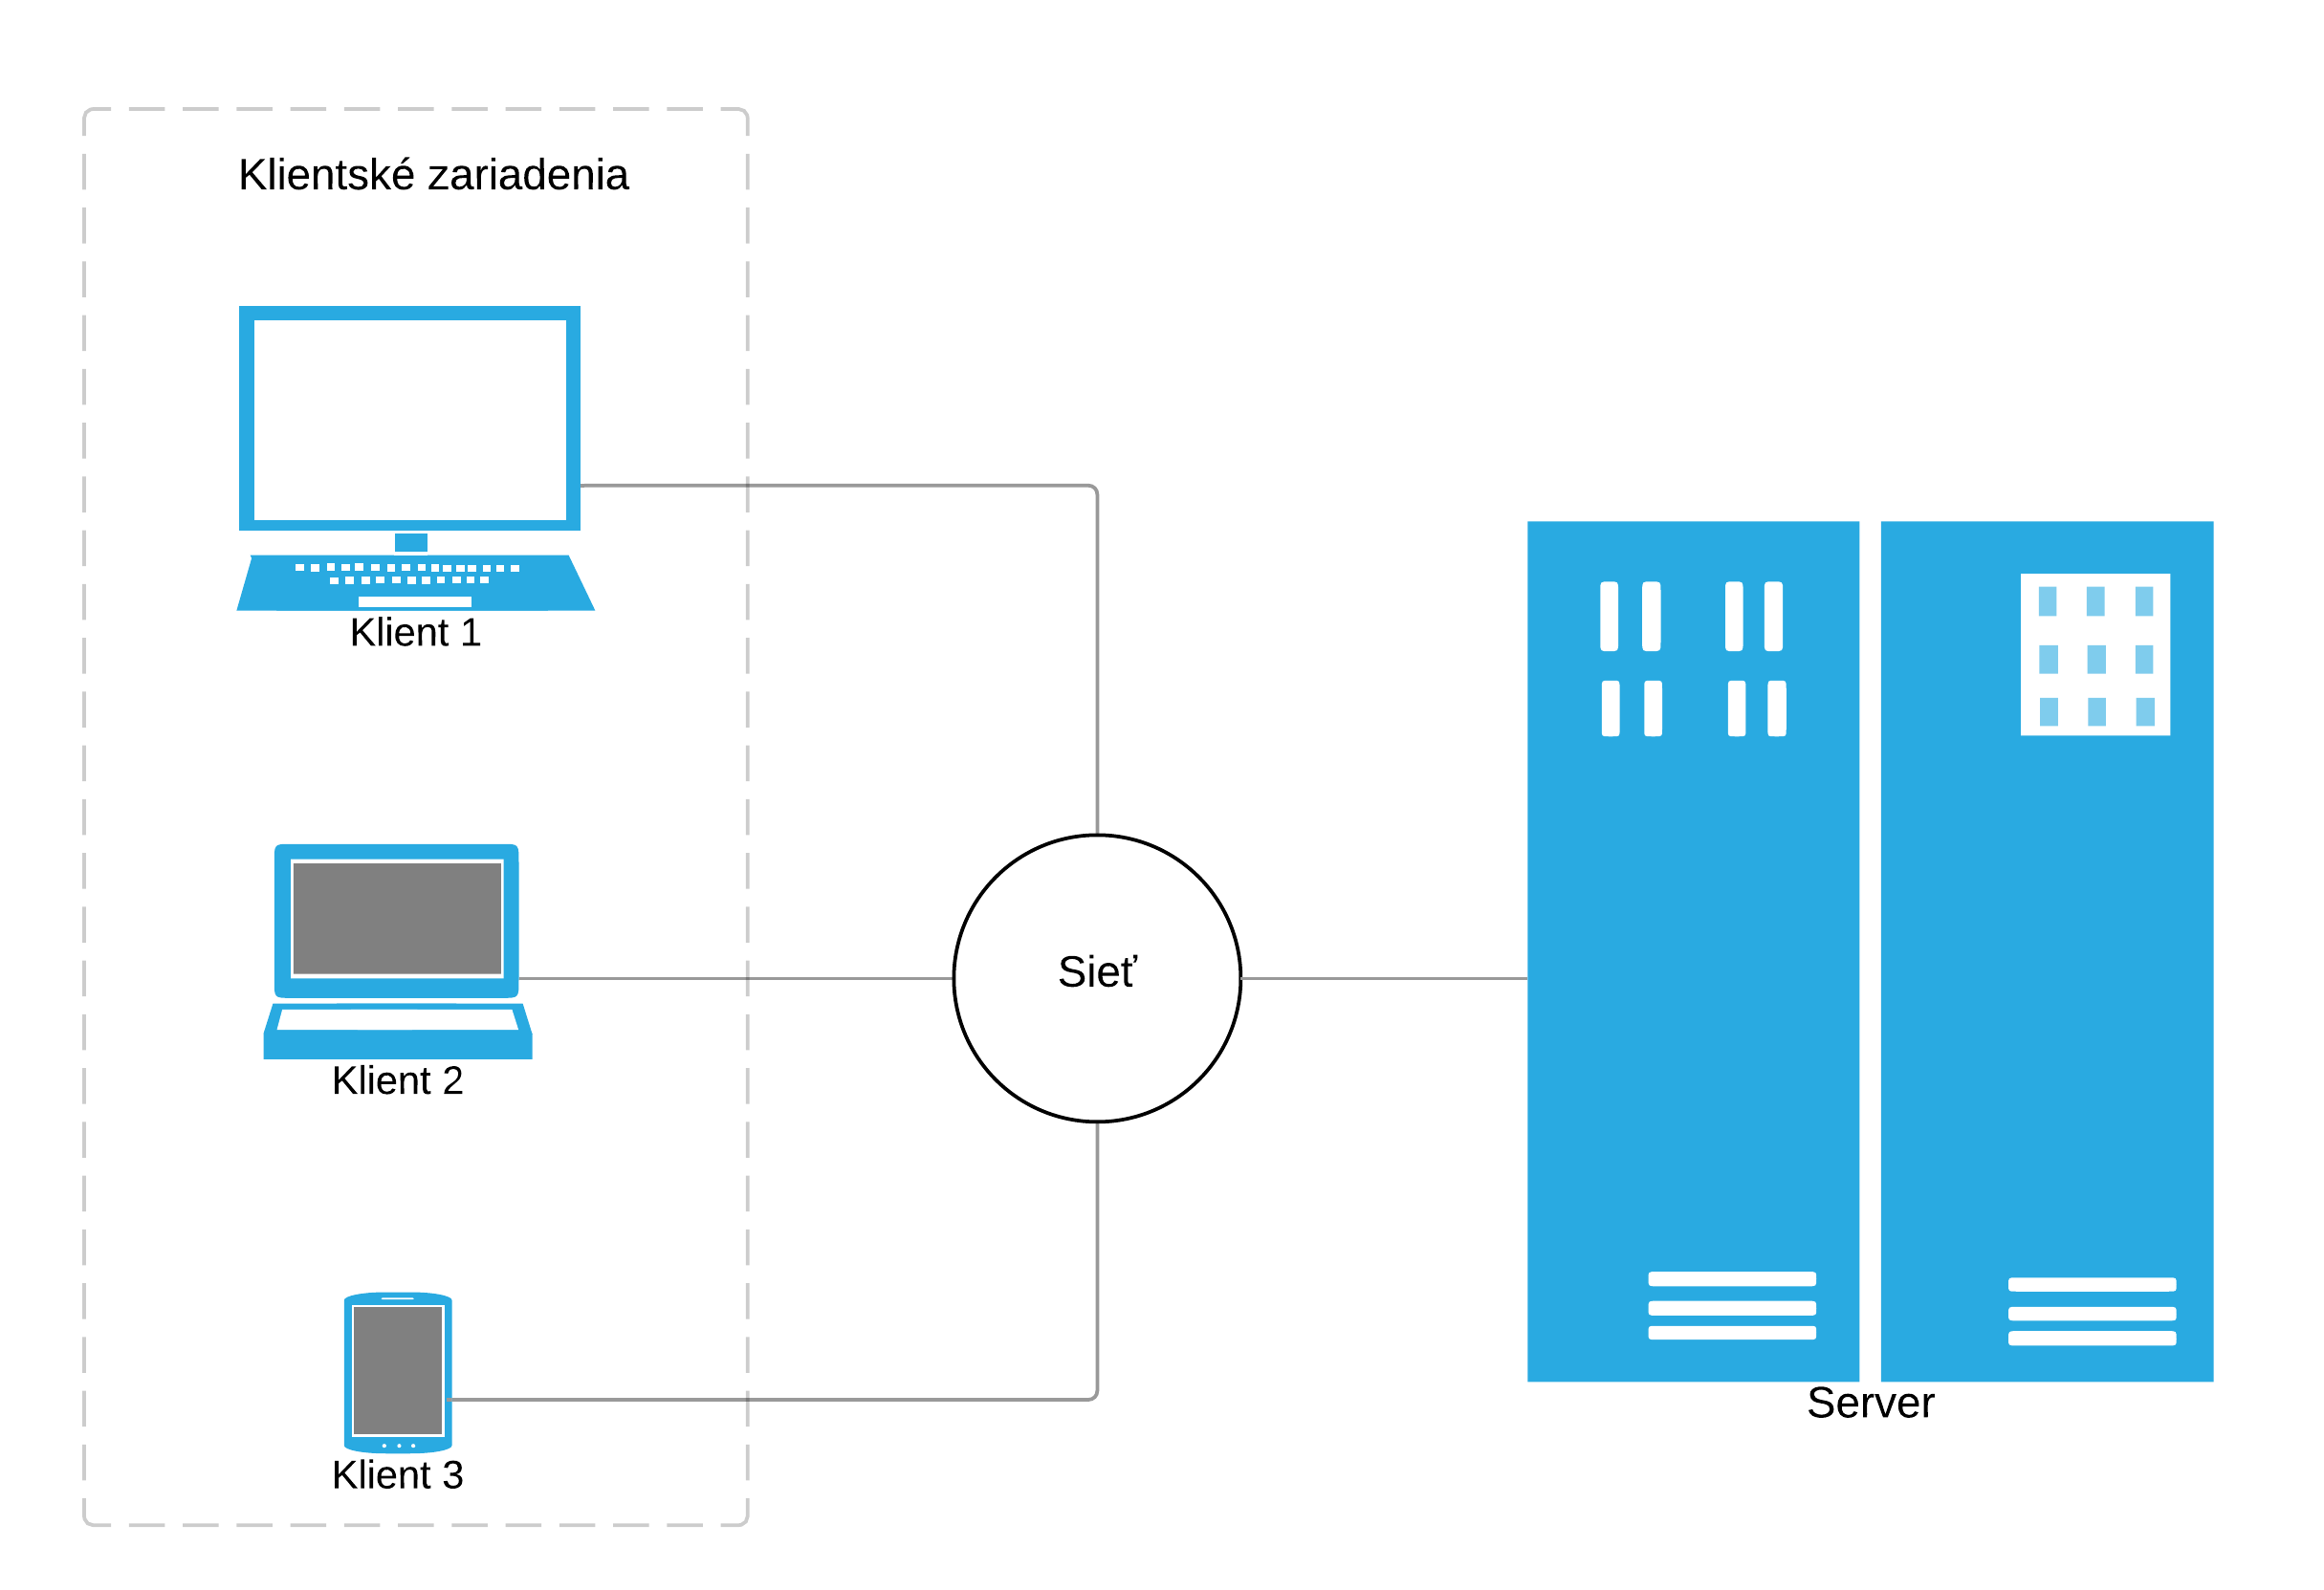
\includegraphics[width=.99\textwidth]{images/C-S-basic.png}
  \caption{Schéma znázorňuje základnú architektúru modelu Klient-Server, zdroj:
  vlastné spracovanie}
  \label{fig:cs-basic}
\end{figure}

\subsection{Klient-Server model}
Pretože Klient-Server model je používaný rôznymi typmi aplikácií bolo nutné
použiť štandardizované protokoly, na základe ktorý ch bude možné komunikovať.
Základné používané protokoly sú: \textit{FTP (File Transfer Protocol)},
\textit{Simple Mail Transfer Protocol (SMTP)} a \textit{Hypertext Transfer
Protocol (HTTP)}. Bližšie sieťové vrstvy a jednotlivé protokoly popisuje
kapitola \ref{ch:net-layers}.

\subsection{Architektúra}
Architektúra modelu Klient-Server sa vo všeobecnosti typicky skladá z troch 
častí:
\begin{itemize}
	\item Aplikačný server
	\item Databázový server
	\item Zariadenie klienta
\end{itemize}
Zároveň Existujú dva základné typy architektúr: 
\begin{itemize}
	\item 2-stupňová \textit{(2-tier)}
	\item 3-stupňová \textit{(3-tier)}
\end{itemize}

\textit{2-tier} architektúra zahrna len zariadenie klienta a databázový server.
U tohoto typu architektúry je aplikácia spustená na zariadení klienta, ktoré sa
následne pripája priamo na server. Zariadenie tak obsluhuje zároveň
\textit{business} logiku aj zobrazovanie aplikácie. Inak tento typ architektúry
nazývame aj tučný klient(\textit{thick client}).

\begin{figure}[H]
  \centering
    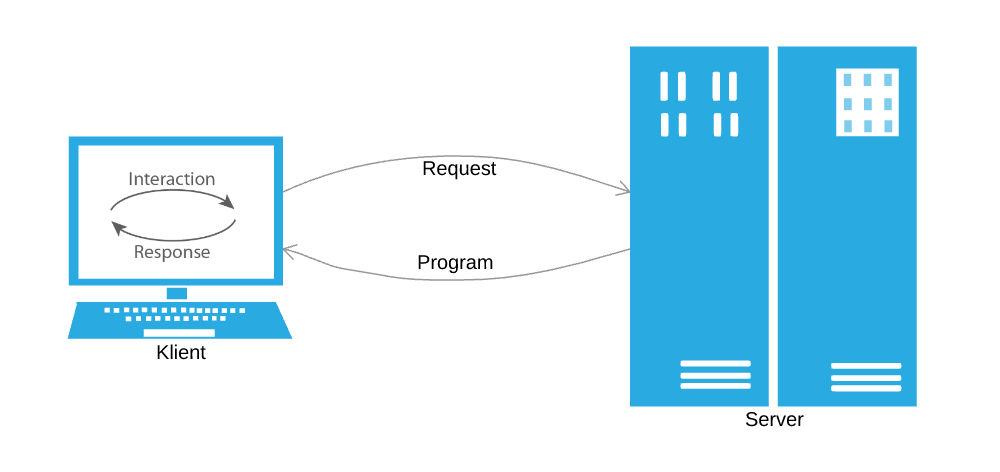
\includegraphics[width=\textwidth]{images/C-S-thick.png}
  \caption{Grafické znázornenie a popis priebehu komunikácie 2-tier architektúry,
  zdroj: vlastné spracovanie}
  \label{fig:cs-thick}
\end{figure}

\textit{3-tier} architektúra, ktorou sa budem zaoberať v tejto práci sa od
\textit{2-tier} líši najmätým, že okrem zariadenia klienta a databázového servera
zahŕňa aj aplikačný server. Tento je následne používaný na obsluhu
\textit{business} logiky aplikácie a komunikáciu s databázou, pričom zariadenie
klienta slúž len na zobrazovanie. Iný názov pre takýto typ architektúry je tenký
klient (\textit{thincient}).

\begin{figure}[H]
  \centering
    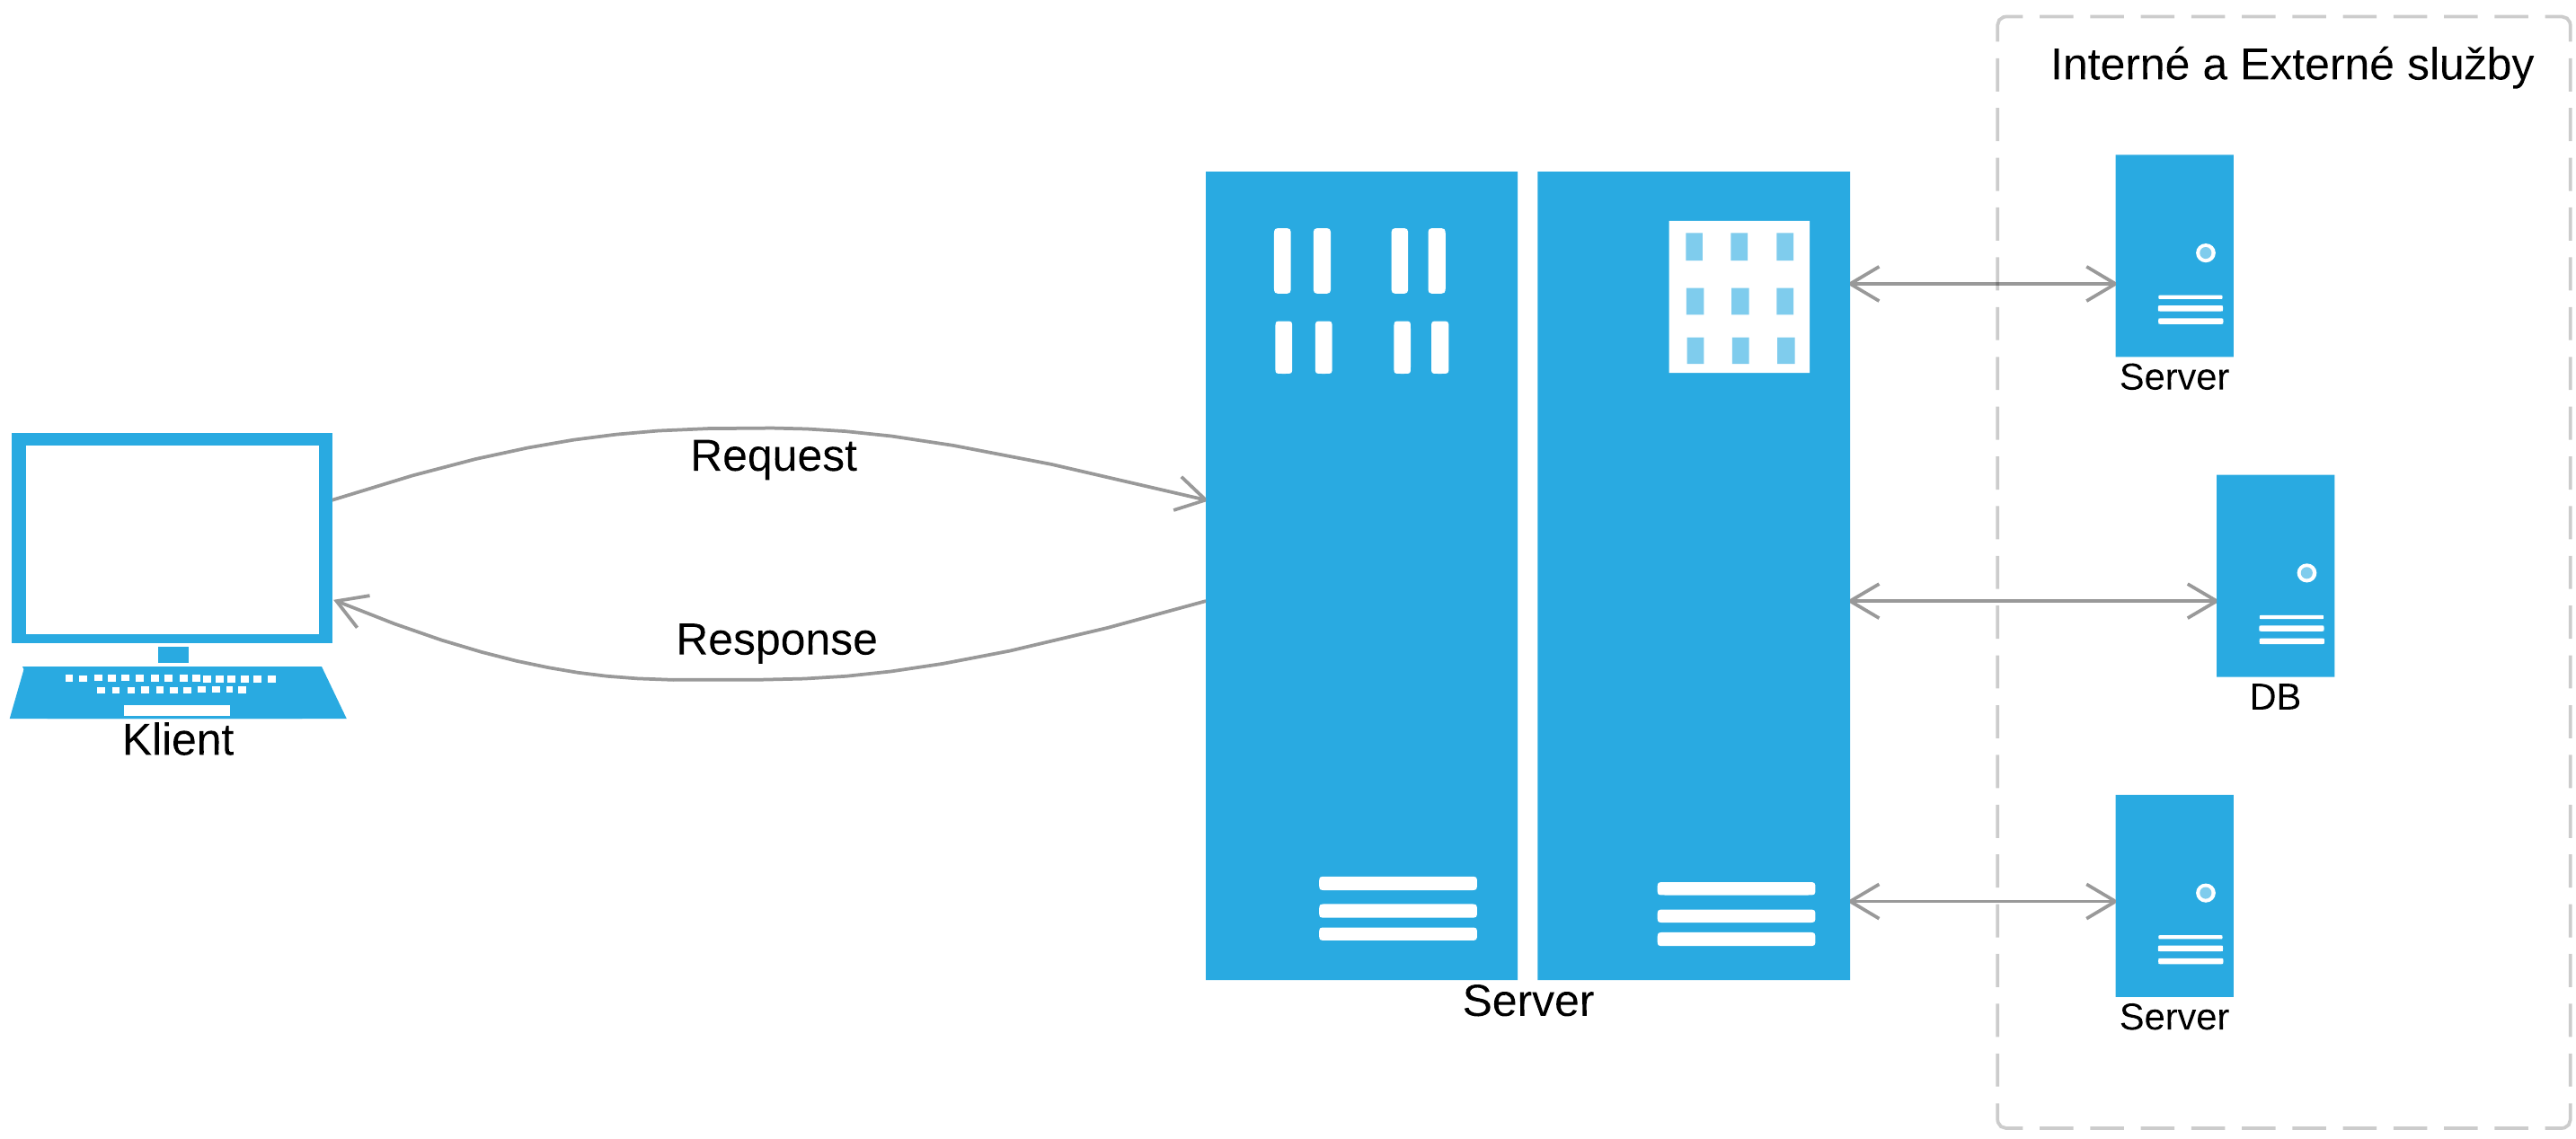
\includegraphics[width=\textwidth]{images/C-S-thin.png}
  \caption{Grafické znázornenie a popis priebehu komunikácie 3-tier architektúry,
  zdroj: vlastné spracovanie}
  \label{fig:cs-thin}
\end{figure}

Nasledujúce kapitoly tejto práce sa budú zaoberať jedným z najdôležitejších
problémov Webových aplikácií, ktorým je identifikácia užívateľa. Najskôr kapitola
\ref{ch:net-layers} analyzuje jednotlivé sieťové vrstvy a protokoly, ktorých
informácie je možné použiť ka následnej identifikácií. Ďalšou časťou je zhrnutie
existujúcich prístupov k rozoznaniu užívateľov v kapitole \ref{ch:existing} a 
popis útokov typu DOS v kapitole \ref{ch:dos}. Najdôležitejšou časťou je však
samozrejme kapitola \ref{ch:footprint}, ktorá popisuje návrh samotného 
algoritmu identifikátoru.

\chapter{Analýza sieťových vrstiev a protokolov}
\label{ch:net-layers}
//TODO - Úvod
\section{Aplikačná vrstva}
\section{Transportná vrstva}
\section{Sieťová vrstva}
\section{Vrstva sieťového rozhrania}

\chapter{Útoky typu \textit{Denial of Service}}
\label{ch:dos}
Jedným z hlavných dôvodov identifikácie užívateľov je prevencia proti útokom. Medzi
najznámejšie z útokov patrí tzv. Denial of Service, ďalej len DoS.

Vo všeobecnosti je za DoS útok považovaná snaha utočníka zabrániť oprávneným
užívateľom v prístupe k informáciám, prípadne službám poskytovateľa. Snahou útočníka
je znefunkčnit pripojenie neustálym narušaním služby serveru, prípadne sieťovej
infraštruktúry, v dôsledku čoho môze dôjsť k čiastočnej, či úplnej strate
internetového pripojenia hostiteľa. 

U distribuovaného DoS útoku (alej len DDoS) môže útočník použiť k útoku na server
počítače klientov. Nad týmito zariadeniami je možné prevziať kontrolu využitím
bezpečnostných chýb alebo nedostatkov. Takto je následne možné donútiť počítač
posielať obrovské množstvo dát na webové servery, prípadne odosielanie nevyžiadanej
pošty na konkrétne e-mailové adresy. Útok sa nazýva "distribuovaný", pretože útočník
používa viac zariadení na začatie útoku denial-of-service.

DoS útok je podobny veľkej skupine ľudí, ktorá sa zhromažďuje pri vstupe do obchodu a
bráni vo vstupe skutočným zákazníkom, ktrých záujmom sú reálne služby.
Utočníci vykonávajúci tieto útoky sa často zameriavajú na webové sluzby a servery,
ktoré su poskytované vysoko profitujúcimi inštitúciami, ako sú napríklad banky,
prípadne platobné brány.

---

DOS - diagram

---

\section{Základne typy a techniky}
Nasledujúce odseky popisuju najpoužívanejšie typy a techniky vykonávania DoS útokov a
identifikujú prostriedky, ktorými je im možné zabrániť.
\subsection{Distribuované DoS útoky}

---

D-DOS - diagram

---

\subsection{Sémantické DoS útoky}
\subsection{Útoky hrubou silou}
\subsection{Nízkoúrovnové DoS utoky}
\subsection{Pokročilé DoS - APDoS}
\subsection{...}
\subsection{Reflekcia}

\chapter{Existujúce prístupy k identifikácií}
\label{ch:existing}
//TODO - Úvod
\section{Využitie sieťovej vrstvy}
//TODO - Úvod
\subsection{Internet Protocol (IP)}
\subsection{Nedostatky}
\section{Aplikačné identifikátory}

\chapter{Tvorba unikátneho identifikátoru}
\label{ch:footprint}
//TODO - Úvod
\section{Možnosti protokolu HTTP}
\section{Možnosti TCP}
\section{Popis Algoritmu}

\section{Záver}

\makeatletter\thesis@blocks@clear\makeatother
\phantomsection %% Print the index and insert it into the
\addcontentsline{toc}{chapter}{\indexname} %% table of contents.
\printindex

\appendix %% Start the appendices.
\chapter{Príloha}
Here you can insert the appendices of your thesis.

\end{document}
